\section{sistemi lineari}

Un sistema lineare omogeneo a coefficienti costanti del primo ordine si
scrive in generale nella forma:
\[
  \vec u'(x) = A \vec u(x)
\]
dove $A$ è una matrice $n\times n$ costante
e la funzione vettoriale incognita sarà
$\vec u \colon \RR\to \RR^n$.
Come per i sistemi lineari algebrici sarà utile, se possibile,
cercare un sistema di riferimento 
in cui la matrice $A$ risulti essere diagonale. Se facciamo il cambio di variabile
\[
  \vec u = M \vec v
\]
tramite una matrice invertibile $M$, si ottiene $\vec u' = (M \vec v)' = M \vec v'$
(si faccia la verifica!... stiamo supponendo che $M$ sia una matrice costante)
e dunque il sistema lineare diventa:
\[
 M \vec v' = A M \vec v
\]
ovvero
\[
  \vec v' = M^{-1} A M \vec v.
\]
A meno di un cambio di variabili potremo quindi sostituire la matrice $A$
con una qualunque matrice simile ad essa: $M^{-1} A M$. In particolare se
la matrice $A$ è diagonalizzabile (ad esempio se gli autovalori di $A$ sono
tutti reali e distinti)
potremo ricondurci a un sistema diagonale:
\[
\begin{cases}
 v_1' = \lambda_1 v_1 \\
      \vdots\\
 v_n' = \lambda_n v_n
\end{cases}
\]
dove $\lambda_1, \dots, \lambda_n$ sono gli autovalori della matrice $A$.
La matrice $M$ del cambio di base avrà come vettori colonna gli autovettori
della matrice $A$, che quindi rappresentano la nuova base. A questo punto
abbiamo $n$ equazioni indipendenti che possono essere risolte
senza difficoltà:
\begin{align*}
  v_1(x) &= c_1 e^{\lambda_1 x}\\
  v_2(x) &= c_2 e^{\lambda_2 x}\\
  &\vdots \\
  v_n(x) &= c_n e^{\lambda_n x}
\end{align*}
con $c_1, \dots, c_n$ costanti arbitrarie.

Se la matrice $A$ non è diagonalizzabile sul campo reale è possibile che
risulti diagonalizzabile nel campo complesso. Più in generale la matrice
potrà essere portata in forma di Jordan. Per brevità non cercheremo di
trattare il caso generale, ma ci concentreremo sul caso $n=2$ che
contiene comunque una casistica piuttosto ampia.

\subsection{sistemi $2\times 2$}

Nel caso $n=2$ sarà comodo usare $t$ come variabile indipendente (al posto di $x$)
e chiamare $x(t)$ e $y(t)$ le due coordinate della funzione vettoriale incognita.
Il sistema che vogliamo trattare sarà quindi della forma:
\[
\begin{cases}
  x'(t) = a\cdot  x(t) + b \cdot y(t)\\
  y'(t) = c\cdot  x(t) + d \cdot y(t).
\end{cases}
\]
dove $a,b,c,d$ sono i coefficienti costanti (reali) della matrice
\[
   A = \begin{pmatrix}
   a & b \\
   c & d
   \end{pmatrix}.
\]
Vedremo che il comportamento del sistema potrà essere classificato in
base agli autovalori della matrice.
Siano $\lambda$ e $\mu$ gli autovalori (eventualmente complessi)
della matrice $A$ cioè gli zeri del polinomio caratteristico:
\[
 P(z)
 = \det (A - z I)
 = z^2 - (a+d) z + ad - bc.
\]

Se gli autovalori sono reali e distinti la matrice è
diagonalizzabile, se $\vec v, \vec w$ sono gli autovettori corrispondenti
agli autovalori $\lambda, \mu$, si potrà quindi fare il cambio
di variabile
\[
\begin{pmatrix} x \\ y \end{pmatrix}
= X \vec v + Y \vec w
\]
tramite il quale le equazioni si separano:
\[
  \begin{cases}
  X' = \lambda X \\
  Y' = \mu Y
  \end{cases}
\]
da cui si ottiene $X = a e^{\lambda t}$, $Y= b e^{\mu t}$
con $a,b\in \RR$ costanti arbitrarie.

Visto che le equazioni a coefficienti costanti sono autonome
sappiamo che una traslazione temporale di una soluzione rimane
una soluzione. Infatti si osserva che
\[
\begin{cases}
  X(t+c) = a e^{\lambda (t+c)} = a e^{\lambda c} e^{\lambda t}, \\
  Y(t+c) = b e^{\mu (t+c)} = b e^{\mu c} e^{\mu t}.
\end{cases}
\]
Questo ci permette di disegnare le traiettorie delle soluzioni
nel piano $(x,y)$. Su tale piano le traslazioni temporali
di una soluzione si rappresentano sulla stessa traiettoria.
Traiettorie diverse non potranno invece mai incontrarsi
per l'unicità della soluzione.

Se $a=b=0$ si ottiene la soluzione nulla $X=0$, $Y=0$ che,
nel piano delle fasi, si rappresenta con un singolo punto
nell'origine. Se $b=0$ le soluzioni sono della forma
$X=a e^{\lambda t}$, $Y=0$ che ha una traiettoria,
nel piano $xy$ lungo la semiretta uscente dall'origine
con direzione $\vec v$
se $a>0$ e con direzione $-\vec v$ se $a<0$.
La soluzione andrà verso $0$ (all'aumentare di $t$)
se $\lambda<0$ e sarà invece uscente da $0$ se $\lambda >0$.
Analogamente si ha una traiettoria sulle due semirette
con direzione $\vec w$ e $-\vec w$ quando $a=0$ e $b\neq 0$.

Se entrambi $a$ e $b$ sono non nulli potremo trovare
l'equazione della traiettoria eliminando la variabile
$t$ nelle
equazioni che rappresentano la soluzione.
Se $X=a e^{\lambda t}$, $Y=b e^{\mu t}$ risulta
\[
  \frac{\abs{b}^\lambda \abs{X}^\mu}{\abs{a}^\mu \abs{Y}^\lambda}
  = \frac{e^{\lambda t \mu}}{e^{\mu t \lambda}} = 1
\]
da cui
\[
 Y = k \abs{X}^{\frac \mu \lambda}
\]
con $k$ costante arbitraria.

\newsavebox{\qrsistemisella}\sbox{\qrsistemisella}{%
  \myqrshortdoclink{sistemi_sella}{sistemi lineari: sella}}
\newsavebox{\qrsisteminodo}\sbox{\qrsisteminodo}{%
  \myqrshortdoclink{sistemi_nodo}{sistemi lineari: nodo}}
\newsavebox{\qrsisteminodoimproprio}\sbox{\qrsisteminodoimproprio}{%
  \myqrshortdoclink{sistemi_nodo_improprio}{sistemi lineari: nodo improprio}}
\newsavebox{\qrsistemistella}\sbox{\qrsistemistella}{%
  \myqrshortdoclink{sistemi_stella}{sistemi lineari: stella}}
\newsavebox{\qrsistemifuoco}\sbox{\qrsistemifuoco}{%
  \myqrshortdoclink{sistemi_fuoco}{sistemi lineari: fuoco}}
\newsavebox{\qrsistemicentro}\sbox{\qrsistemicentro}{%
  \myqrshortdoclink{sistemi_centro}{sistemi lineari: centro}}
\begin{figure}
\centering
 \begin{subfigure}{5cm}
  %\centering
  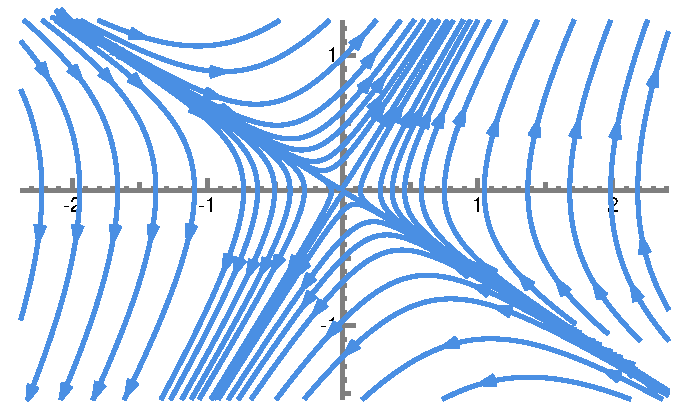
\includegraphics[width=0.75\textwidth]{sistemi_sella.pdf}
  \caption[1a]{sella (instabile)}
 \end{subfigure}
 \begin{subfigure}{5cm}
  %\centering
  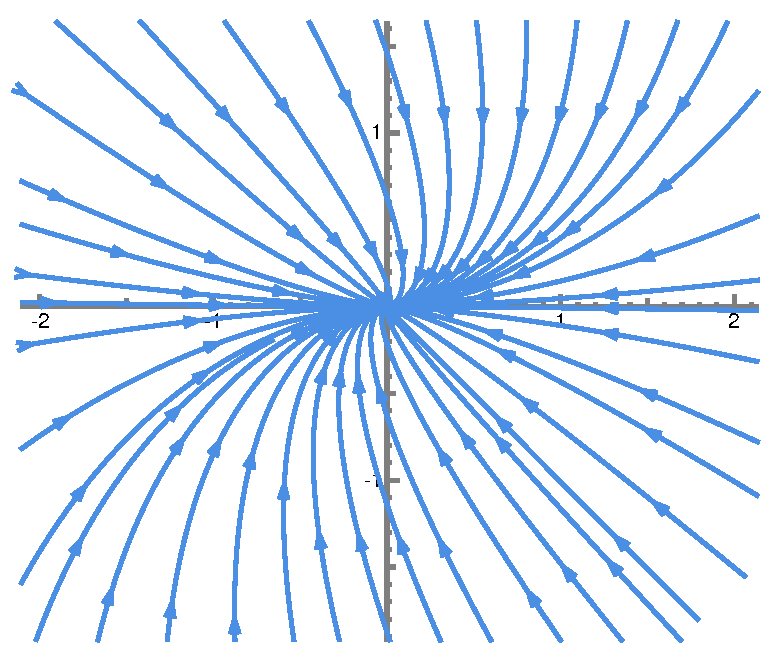
\includegraphics[width=0.75\textwidth]{sistemi_nodo.pdf}
  \caption{nodo stabile}
 \end{subfigure}
 \begin{subfigure}{5cm}
 \centering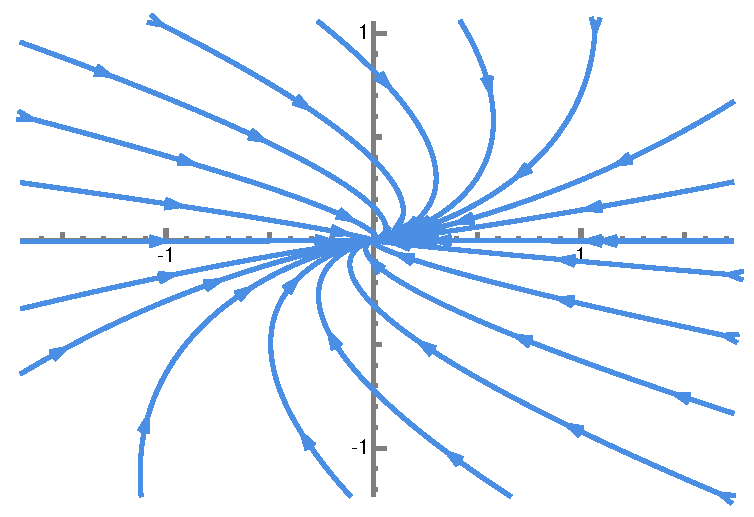
\includegraphics[width=0.75\textwidth]{sistemi_nodo_improprio.pdf}
  \caption{nodo improprio stabile}
 \end{subfigure}
 \begin{subfigure}{5cm}
  \centering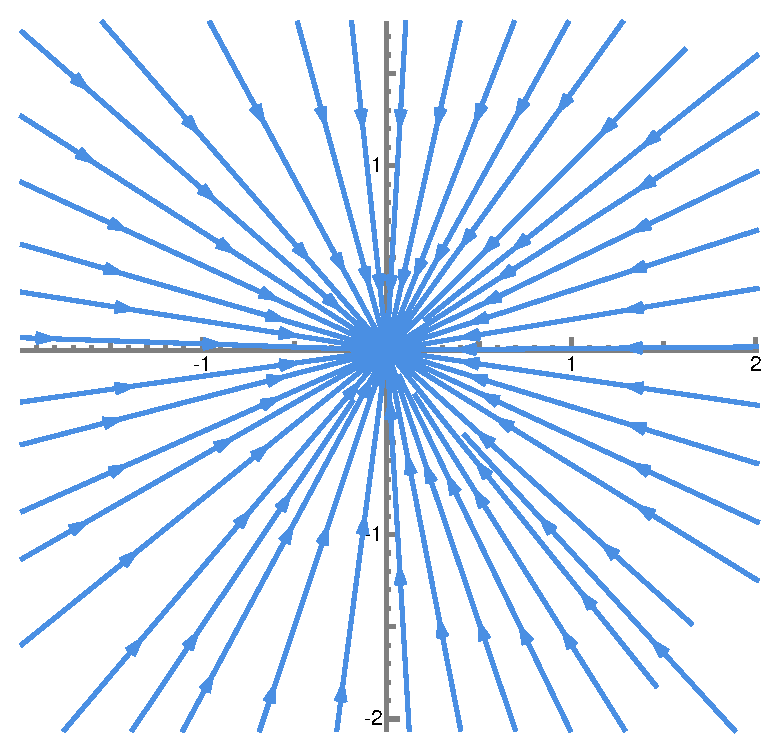
\includegraphics[width=0.75\textwidth]{sistemi_stella.pdf}
  \caption{stella stabile}
 \end{subfigure}
 \begin{subfigure}{5cm}
  \centering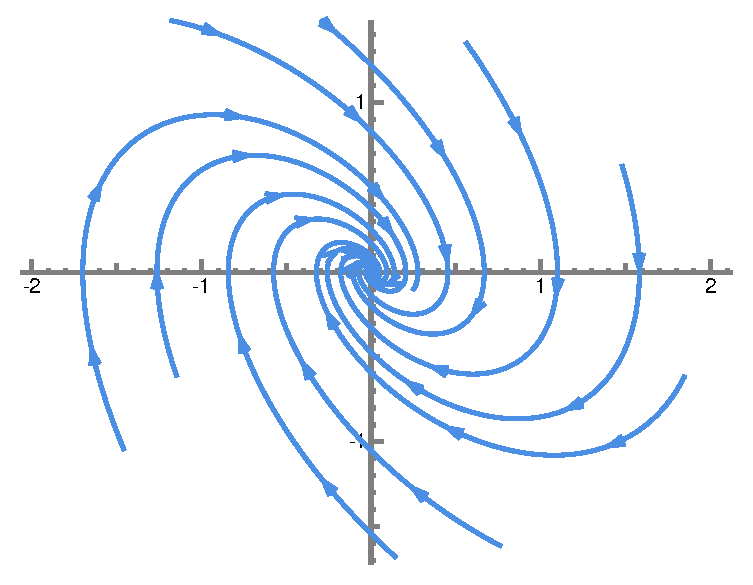
\includegraphics[width=0.75\textwidth]{sistemi_fuoco.pdf}
  \caption{fuoco stabile}
 \end{subfigure}
 \begin{subfigure}{5cm}
  \centering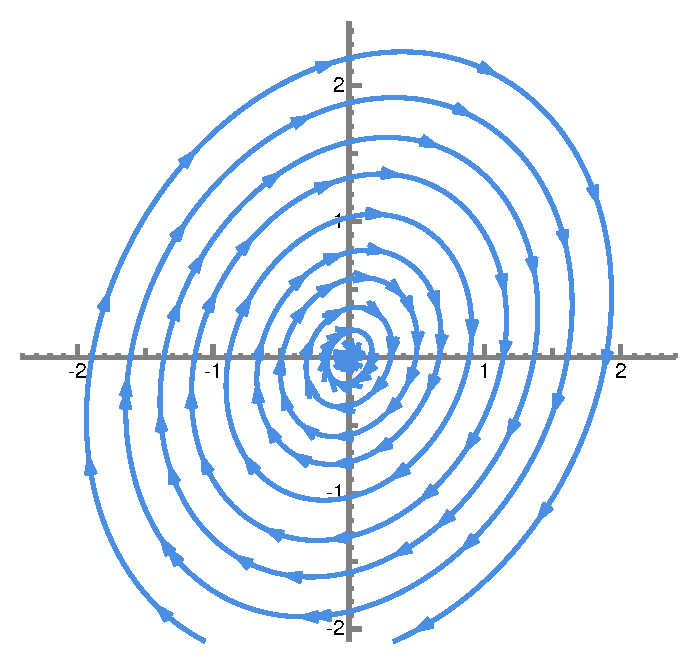
\includegraphics[width=0.75\textwidth]{sistemi_centro.pdf}
  \caption{centro (stabile)}
 \end{subfigure}
 \caption{\\%
 \usebox{\qrsistemisella} \usebox{\qrsisteminodo}\\
 \usebox{\qrsisteminodoimproprio} \usebox{\qrsistemistella}\\
 \usebox{\qrsistemifuoco} \usebox{\qrsistemicentro}
 }
\end{figure}

Se i segni di $\lambda$ e $\mu$ sono opposti,
si ottiene una configurazione chiamata
\emph{sella}%
\mymargin{sella}\index{sella} (si veda figura).
Lungo l'autovettore con autovalore negativo
ci sarà convergenza verso l'origine, ma questa
convergenza è instabile in quanto ogni altra
curva tenderà invece a essere deviata
e a tendere asintoticamente verso la direzione
dell'autovettore con autovalore positivo.

Se $\lambda$ e $\mu$ sono entrambi negativi si
ha un \emph{nodo stabile}%
\mymargin{nodo stabile}\index{nodo!stabile} in cui tutte le
curve convergono verso l'origine (soluzione
attrattiva). Se invece $\lambda$ e $\mu$
sono entrambi positivi le curve
saranno percorse in senso inverso e saranno
uscenti dall'origine: si avrà allora
un \emph{nodo instabile}%
\mymargin{nodo instabile}\index{nodo!instabile}.

Se gli autovalori sono coincidenti $\lambda=\mu$
e se la matrice è diagonalizzabile allora
la matrice è diagonale, tutti i vettori sono
autovettori quindi in ogni direzione c'è
una traiettoria rettilinea.
La configurazione si
chiama \emph{stella}%
\mymargin{stella}\index{stella} (stabile o instabile a seconda
del segno negativo o positivo).

Se gli autovalori sono coincidenti $\lambda = \mu$ e la matrice
non è diagonalizzabile consideriamo l'autovettore (unico)
$\vec u$ con $A \vec u = \lambda \vec u$
e prendiamo un qualunque vettore $\vec w$
indipendente da $\vec u$. Allora si avrà
\[
  A \vec w = \alpha \vec u + \beta \vec w.
\]
Certamente $\alpha \neq 0$ altrimenti $\vec w$
sarebbe un autovettore e la matrice sarebbe diagonalizzabile.
Consideriamo allora $\vec v = \vec w / \alpha$
cosicché si ha $A \vec v = \vec u + \frac{\beta}{\alpha} \vec w$.
Nella base $\vec u, \vec v$ la matrice $A$ diventa
triangolare, e sulla diagonale troviamo i valori $\lambda$
e $\frac{\beta}{\alpha}$.
Ma allora $\frac{\beta}{\alpha} = \lambda$ in quanto sulla diagonale
abbiamo solo gli autovalori. Dunque se $X,Y$ sono le coordinate nel
sistema $\vec u, \vec v$, il sistema di equazioni diventa:
\[
\begin{cases}
X' = \lambda X + Y \\
Y' = \lambda Y.
\end{cases}
\]
Dalla seconda equazione si ottiene quindi $Y = a e^{\lambda t}$
con $a\in \RR$ costante arbitraria
e sostituendo nella prima si ottiene l'equazione
\[
  X' - \lambda X = a e^{\lambda t}
\]
che può essere risolta trovando una seconda costante arbitraria $b\in \RR$ e
\[
  X = (at+b) e^{\lambda t}.
\]
Se $a=0$ una traiettoria con $Y=0$ cioè nella direzione dell'unico autovettore.
Se $\lambda <0$ tale traiettoria sarà convergente a $0$ altrimenti sarà divergente.
Se $a\neq 0$ possiamo eliminare $t$ ponendo:
\[
  t = \frac 1 \lambda \ln \frac{Y}{a}
\]
e quindi
\[
  X = \enclose{\frac{a}{\lambda} \ln \frac{Y}{a}+ b} \frac{Y}{a}
  =  \frac{Y}{\lambda}\ln \frac{Y}{a}+ \frac{b}{a}Y.
\]
Studiando il grafico di questa funzione si ottengono qualitativamente
le curve disegnate in figura: la configurazione si chiama \emph{nodo improprio}%
\mymargin{nodo improprio}\index{nodo improprio}.
Come per i nodi le traiettorie convergono all'origine se $\lambda < 0$ e
divergono se $\lambda >0$.

Proviamo a trattare il caso, più interessante,
degli autovalori complessi. Se la matrice è a coefficienti
reali gli autovalori, quando
non reali, saranno certamente complessi coniugati:
\[
  \lambda = \alpha - i \beta,
  \qquad
  \mu = \alpha + i \beta
\]
con $\alpha,\beta\in \RR$, $\beta\neq 0$.

Sia $\vec v + i \vec w$ un autovettore complesso relativo
all'autovalore $\alpha - i \beta$.
Allora si ha
\[
 A\vec v + i A \vec w
 = A(\vec v + i \vec w)
 = (\alpha - i \beta)(\vec v + i \vec w)
 = \alpha \vec v + \beta \vec w +i(-\beta \vec v + \alpha \vec w).
\]
Uguagliando parte reale e parte immaginaria si trova
\[
  A \vec v = \alpha \vec v + \beta \vec w,
  \qquad
  A \vec w = -\beta \vec v + \alpha \vec w.
\]
A questo punto non è difficile verificare che $\vec v - i \vec w$
è un autovettore relativo all'autovalore coniugato $\alpha + i\beta$.
Visto che $\vec v\pm i\vec w$ sono due autovettori con autovalori
distinti sicuramente sono vettori indipendenti.
Dunque anche $\vec v$ e $\vec w$
(che si ottengono come multipli di somma e differenza)
sono vettori indipendenti
(stavolta reali).
Se $X,Y$ sono le coordinate nella base $\vec v$, $\vec w$, l'equazione
differenziale diventa:
\[
\begin{cases}
 X' = \alpha X - \beta Y \\
 Y' = \beta X + \alpha Y.
\end{cases}
\]
Si ha allora%
\mynote{Si potrebbe osservare che la matrice
$\begin{pmatrix}\alpha&-\beta\\ \beta & \alpha\end{pmatrix}$
è la matrice che rappresenta la moltiplicazione
complessa per il numero $\alpha + i\beta$. Dunque chiamando $Z=X+iY$
il sistema si potrebbe scrivere nella forma $Z'=(\alpha +i\beta)Z$
e si potrebbe quindi osservare immediatamente
che la soluzione deve essere della forma $Z = c e^{(\alpha+i\beta)t}$
con $c$ costante complessa. Ponendo poi $c=\rho e^{i\theta}$
si ottiene il risultato.}
\[
 X'' = \alpha X' - \beta Y'
 = \alpha X' - \beta (\beta X + \alpha Y)
\]
da cui, usando $\beta Y = \alpha X - X'$ possiamo eliminare la variabile $Y$
e ottenere una equazione del secondo ordine in $X$:
\[
 X'' = \alpha X' - \beta^2 X - \alpha (\alpha X - X')
  = 2 \alpha X' - (\alpha^2+\beta^2) X
\]
ovvero
\[
 X'' - 2 \alpha X' + (\alpha^2 + \beta^2) X = 0.
\]
Risolvendo questa equazione del secondo ordine ci si accorge
che le radici del polinomio caratteristico sono proprio $\alpha \pm i \beta$
e quindi le soluzioni si scrivono nella forma
\[
X = e^{\alpha t}(a \cos \beta t + b \sin \beta t)
\]
da cui
\begin{align*}
\beta Y
&= \alpha X - X'\\
& = \alpha e^{\alpha t}(a \cos \beta t + b \sin \beta t) \\
&\quad - \alpha e^{\alpha t}(a\cos \beta t + b \sin \beta t)
  - e^{\alpha t}(-\beta a \sin \beta t + b \beta \cos \beta t) \\
 &= \beta e^{\alpha t}(a\sin \beta t - b \cos \beta t).
\end{align*}
Dunque, ponendo $\rho=\sqrt{a^2+b^2}$ e scegliendo $\theta$
tale che $\cos \theta = \frac a \rho$ e $\sin \theta = - \frac b \rho$,
si ha
\[
  \begin{cases}
   X = \rho e^{\alpha t} \cos(\beta t + \theta),\\
   Y = \rho e^{\alpha t} \sin(\beta t + \theta).
  \end{cases}
\]
Se $\alpha \neq 0$ le traiettorie corrispondenti formano delle spirali
ellittiche che si avvitano nella direzione che porta il vettore $\vec v$ verso
il vettore $\vec w$. Se $\alpha < 0$ le spirali convergono verso l'origine del
sistema: avremo un \emph{fuoco stabile}%
\mymargin{fuoco stabile}\index{fuoco stabile}. Se $\alpha >0$ le orbite
divergono chiameremo la configurazione un \emph{fuoco instabile}%
\mymargin{fuoco instabile}\index{fuoco instabile}.
Se $\alpha = 0$ le traiettorie sono delle ellissi concentriche,
le soluzioni sono quindi periodiche e la configurazione
si chiama \emph{centro}%
\mymargin{centro}\index{centro}.

Se almeno uno dei due autovalori è nullo il comportamento del sistema è degenere,
si hanno delle soluzioni banali che non andremo a investigare.

\subsection{matrice esponenziale}

Per risolvere, in astratto, il sistema $n\times n$ del primo ordine, 
lineare omogeneo a coefficienti costanti
\[
  \vec u' = A \vec u
\]
introduciamo le seguenti nozioni.

Sia $A$ una matrice quadrata $n\times n$. Definiamo la norma (norma
operatoriale) di $A$ come segue:
\[
  \Abs{ A } = \sup_{\abs{\vec v} \le 1} \abs{A\vec v}
\]
dove $\abs{ \vec v} = \sqrt{v_1^2+ \dots + v_n^2}$ è l'usuale norma del
vettore $\vec v\in \RR^n$.
Osserviamo che $\vec v\mapsto A\vec v$ è una funzione
continua e che $\ENCLOSE{\vec v\colon \abs{ \vec v} \le 1}$ è un insieme
compatto, dunque il $\sup$ nella definizione è in realtà un $\max$.

Per le proprietà del $\sup$ si ha:
\[
  \abs{A\vec v} \le \Abs{ A }\, \abs{ v }
\qquad\text{e}\qquad
  \Abs{ A B } \le \Abs{ A } \, \Abs{ B }.
\]
Dunque possiamo affermare il valore assoluto di ogni elemento di una
matrice si stima con la norma della matrice: $\abs{ A_{ij}} \le
\Abs{ A }$, infatti:
\[
  \abs{ A_{ij} } = \abs{ (A \vec e_j)_i} \le \abs{ A e_j}
  \le \Abs{ A }
\]
(dove $\vec e_j$ è il $j$-esimo vettore della base canonica di $\RR^n$).

Se $A_k$ è una successione di matrici, diremo che $A_k\to A$ se ogni
elemento della matrice $A_k$ converge al corrispondente elemento della
matrice $A$: $(A_k)_{ij} \to A_{ij}$. Questo corrisponde a considerare
la matrice $n\times n$ come un vettore dello spazio $\RR^{(n^2)}$.

Se $A(t)$ è una funzione a valori matrici (ovvero una matrice i cui
elementi sono funzioni di $t$), si potrà farne la derivata
come si fa per le funzioni vettoriali: $(A'(t))_{ij} = (A_{ij}(t))'$
cioè componente per componente. Le usuali regole per le derivate
valgono anche per le matrici, in particolare non è difficile
verificare (si espliciti la definizione del prodotto di matrici) che
\[
 (A(t)B(t))' = A'(t) B(t) + A(t) B'(t)
\]
dove, puntualizziamo, è importante mantenere i prodotti nell'ordine
giusto, in quanto il prodotto di matrici può non essere commutativo.

Se $A$ è una matrice quadrata, si definisce la matrice potenza $A^k$
per ogni $k$ naturale, mediante le proprietà
\[
  A^0 = I, \qquad A^{k+1} = A^kA.
\]
(se $A$ è invertibile si possono definire anche le potenze negative
$A^{-k}=(A^{-1})^k = (A^k)^{-1}$).

Definiamo allora la matrice esponenziale di $A$:
\[
  e^A = \sum_{k=0}^{+\infty} \frac{A^k}{k!}.
\]
Per dare significato a questa definizione dobbiamo verificare che la
serie appena scritta sia convergente. Cioè dobbiamo verificare che per
ogni coppia di indici $ij$ sia convergente la serie numerica:
\[
 \sum_{k=0}^{+\infty} \frac{(A^k)_{ij}}{k!}.
\]
Per quanto detto prima sappiamo che
$\abs{(A^k)_{ij}} \le \Abs{A^k} \le \Abs{A}^k$.
Dunque la serie in questione è
assolutamente convergente in quanto il suo valore assoluto si stima
con la serie
\[
 \sum_{k=0}^{+\infty} \frac{\Abs{ A}^k}{k!} = e^{\Abs{ A}}
\]
che è convergente. La definizione della matrice $e^A$ è dunque
ben posta e si ha
\[
 \Abs{ e^A} \le e^{\Abs{ A }}.
\]

\begin{theorem}[proprietà dell'esponenziale matrice]
Siano $A$ e $B$ matrici quadrate $n\times n$ e $t$ uno scalare.
Valgono le seguenti proprietà:
\begin{enumerate}
\item $e^0 = I$ (dove $0$ è la matrice nulla $n\times n$ ed $I$ è la
  matrice identità con le stesse dimensioni);
\item se $AB=BA$ allora $e^A B = B e^A$;
\item $(e^{tA})' = A e^{tA}$;
\item $e^{-A} = (e^A)^{-1}$ (in particolare la matrice esponenziale è
  sempre invertibile);
\item se $\vec u(t)$ è una funzione a valori in $\RR^n$ che soddisfa
  l'equazione differenziale $\vec u'(t) = A\vec u(t)$ allora
  $\vec u(t) = e^{tA} \vec u(0)$;
\item se $AB=BA$ allora $e^{A+B} = e^A e^B$;
\item se $A$ è invertibile allora $e^{ABA^{-1}} = Ae^BA^{-1}$;
\item se $A$ è la matrice diagonale $A = \diag(\lambda_1, \dots, \lambda_n)$,
allora $e^A$
 è pure una matrice diagonale con $e^A = \diag(e^{\lambda_1},\dots, e^{\lambda_n})$;
\item se $A$ è una matrice triangolare con la diagonale nulla (cioè
  $A_{ij}=0$ se $i\ge j$) allora $e^A = \sum_{k=0}^n \frac{A^k}{k!}$
  (basta sommare i primi $n+1$ termini);
\item se $B$ è una matrice triangolare (cioè $B_{ij}=0$ se $i > j$)
  allora $B = D + A$ con $D$ matrice diagonale e $A$ matrice
  triangolare con la diagonale nulla e quindi $e^B = e^De^A$ si può
  calcolare riconducendosi ai punti precedenti.
\end{enumerate}
\begin{proof}
1. Per quanto riguarda $e^0$ osserviamo che per definizione $0^0=I$
mentre $0^k=0$ se $k>0$. Dunque direttamente dalla definizione si
ottiene $e^0=I$.

2. Se $AB=BA$ osserviamo che si ha anche $A^k B=B A^k$ (la matrice $B$
commuta con ogni fattore del prodotto $A^k$). Dunque:
\[
 \sum_{k=0}^N \frac{A^k}{k!} B = B \sum_{k=0}^N \frac{A^k}{k!}
\]
e passando al limite $N\to \infty$ si ottiene $e^A B = B e^A$.

3. Per calcolare la derivata di $e^{tA}$ vogliamo dimostrare che la serie
che definisce $e^{tA}$ converge totalmente quando $t$ varia in un
qualunque intervallo limitato. Poniamo allora $t\in [-M,M]$. Si ha:
\[
  \sup_{t\in[-M,M]}\frac{\Abs{ (tA)^k}}{k!}
  = \sup_{t\in[-M,M]}\frac{\abs{ t}^k \Abs{ A^k}}{k!}
  \le \frac{M^k\Abs{ A}^k}{k!}
\]
la cui serie è convergente qualunque sia $M\in \RR$. Dunque la serie
che definisce $e^{tA}$ è una serie di funzioni continue e derivabili
che converge totalmente su ogni intervallo limitato. Possiamo quindi
derivare la serie termine a termine:
\[
(e^{tA})' = \sum_{k=0}^\infty \frac{((tA)^k)'}{k!}
 = \sum_{k=1}^\infty \frac{kt^{k-1} A^k}{k!}
 = A \sum_{k=1}^\infty \frac{t^{k-1}A^{k-1}}{(k-1)!}
 = A e^{tA}.
\]

4. Dimostriamo ora che $U(t) = e^{tA}e^{-tA}=I$ per ogni $t$. Si ha:
\[
 U'(t) = A e^{tA}e^{-tA} + e^{tA}(-A)e^{-tA}
       = A e^{tA}e^{-tA} - A e^{tA}e^{-tA} = 0
\]
($Ae^{tA} = e^{tA}A$ in quanto $A$ e $tA$ commutano).
Dunque $U'(t)=0$ cioè $U(t)$ è costante ovvero $U(t)=U(0)$. Ma $U(0)=I$
in quanto $e^0=I$ e quindi $U(t)=I$ per ogni $t$.

5. Prendiamo l'equazione $\vec u' = A\vec u$, moltiplicando a sinistra per
$e^{-tA}$ l'equazione diventa
$e^{-tA} \vec u' - e^{-tA} A \vec u=0$ cioè $(e^{-tA} \vec u)' = 0$. Questo significa
che la funzione $e^{-tA}\vec u = c$ costante e moltiplicando a sinistra per
$e^{tA}$ si ottiene dunque $\vec u = e^{tA}c$ come volevasi dimostrare.

6. Per dimostrare la proprietà $e^{A+B}=e^A e^B$ consideriamo la quantità
$U(t) = e^{-t(A+B)} e^{tA} e^{tB}$. Se dimostriamo che $U$ è costante,
visto che $\vec u(0)=I$ si avrà anche $U(1)=I$ che è equivalente a quanto
vogliamo dimostrare. Dunque verifichiamo che la derivata è nulla,
sfruttando l'ipotesi $AB=BA$ che ci permette di far commutare i prodotti:
\begin{align*}
U'(t) & = -(A+B)e^{-t(A+B)} e^{tA} e^{tB} + e^{-t(A+B)}Ae^{tA}e^{tB} +
e^{-t(A+B)}e^{tA} B e^{tB} \\
& = [-(A+B) + A + B] U(t) = 0.
\end{align*}

7. Se $A$ è invertibile allora $(ABA^{-1})^k = ABA^{-1}ABA\dots ABA^{-1}
= AB^k A^{-1}$. Dunque nelle somme parziali della serie che definisce l'esponenziale
$e^{ABA^{-1}}$ si può raccogliere $A$ a sinistra e $A^{-1}$ a destra e
al centro rimane la serie che definisce $e^B$.

8. Se la matrice $A$ è diagonale con $A_{ii}=\lambda_i$ allora $A^k$
risulta essere una matrice diagonale con $(A^k)_{ii} =
\lambda_i^k$. Dunque nella definizione di esponenziale $e^A$ i termini
della serie sono tutte matrici diagonali, e sulla diagonale compare la
serie che definisce l'esponenziale $e^{\lambda_i}$.

9. Se $A$ è una matrice triangolare con $A_{ij}=0$ quando $i\ge j$, si
osserva che $A^2$ avrà degli zeri anche sopra la diagonale:
$(A^2)_{ij}=0$ quando $i+1\ge j$ (si applichi la definizione di
prodotto, riga per colonna). Nelle moltiplicazioni successive $A^3,
A^4,\dots$ si aggiungerà sempre una diagonale di zeri finché la matrice non
si annulla completamente $A^n=0$. Dunque la serie che definisce $e^A$
contiene solo un numero finito di termini (i primi $n+1$) e può essere
calcolata esplicitamente.

10. L'ultima proprietà è una osservazione che non richiede dimostrazione.
\end{proof}
\end{theorem}

